


\begin{frame}{Neural Networks}
\begin{columns}
    \begin{column}{0.5\textwidth}
    \begin{itemize}
        \item Built of layers of simple processors called nodes
        \item Each node is connected to each node in the surrounding layers
        \item The connection is built by a linear function with a weight $\omega$ and a bias $b$ 
        and a non linear activation function $\sigma$
        \item Learning is accomplished by backpropagation and a step optimizer
    \end{itemize}
    \end{column}
    \begin{column}{0.5\textwidth}
    \begin{figure}
        \centering
        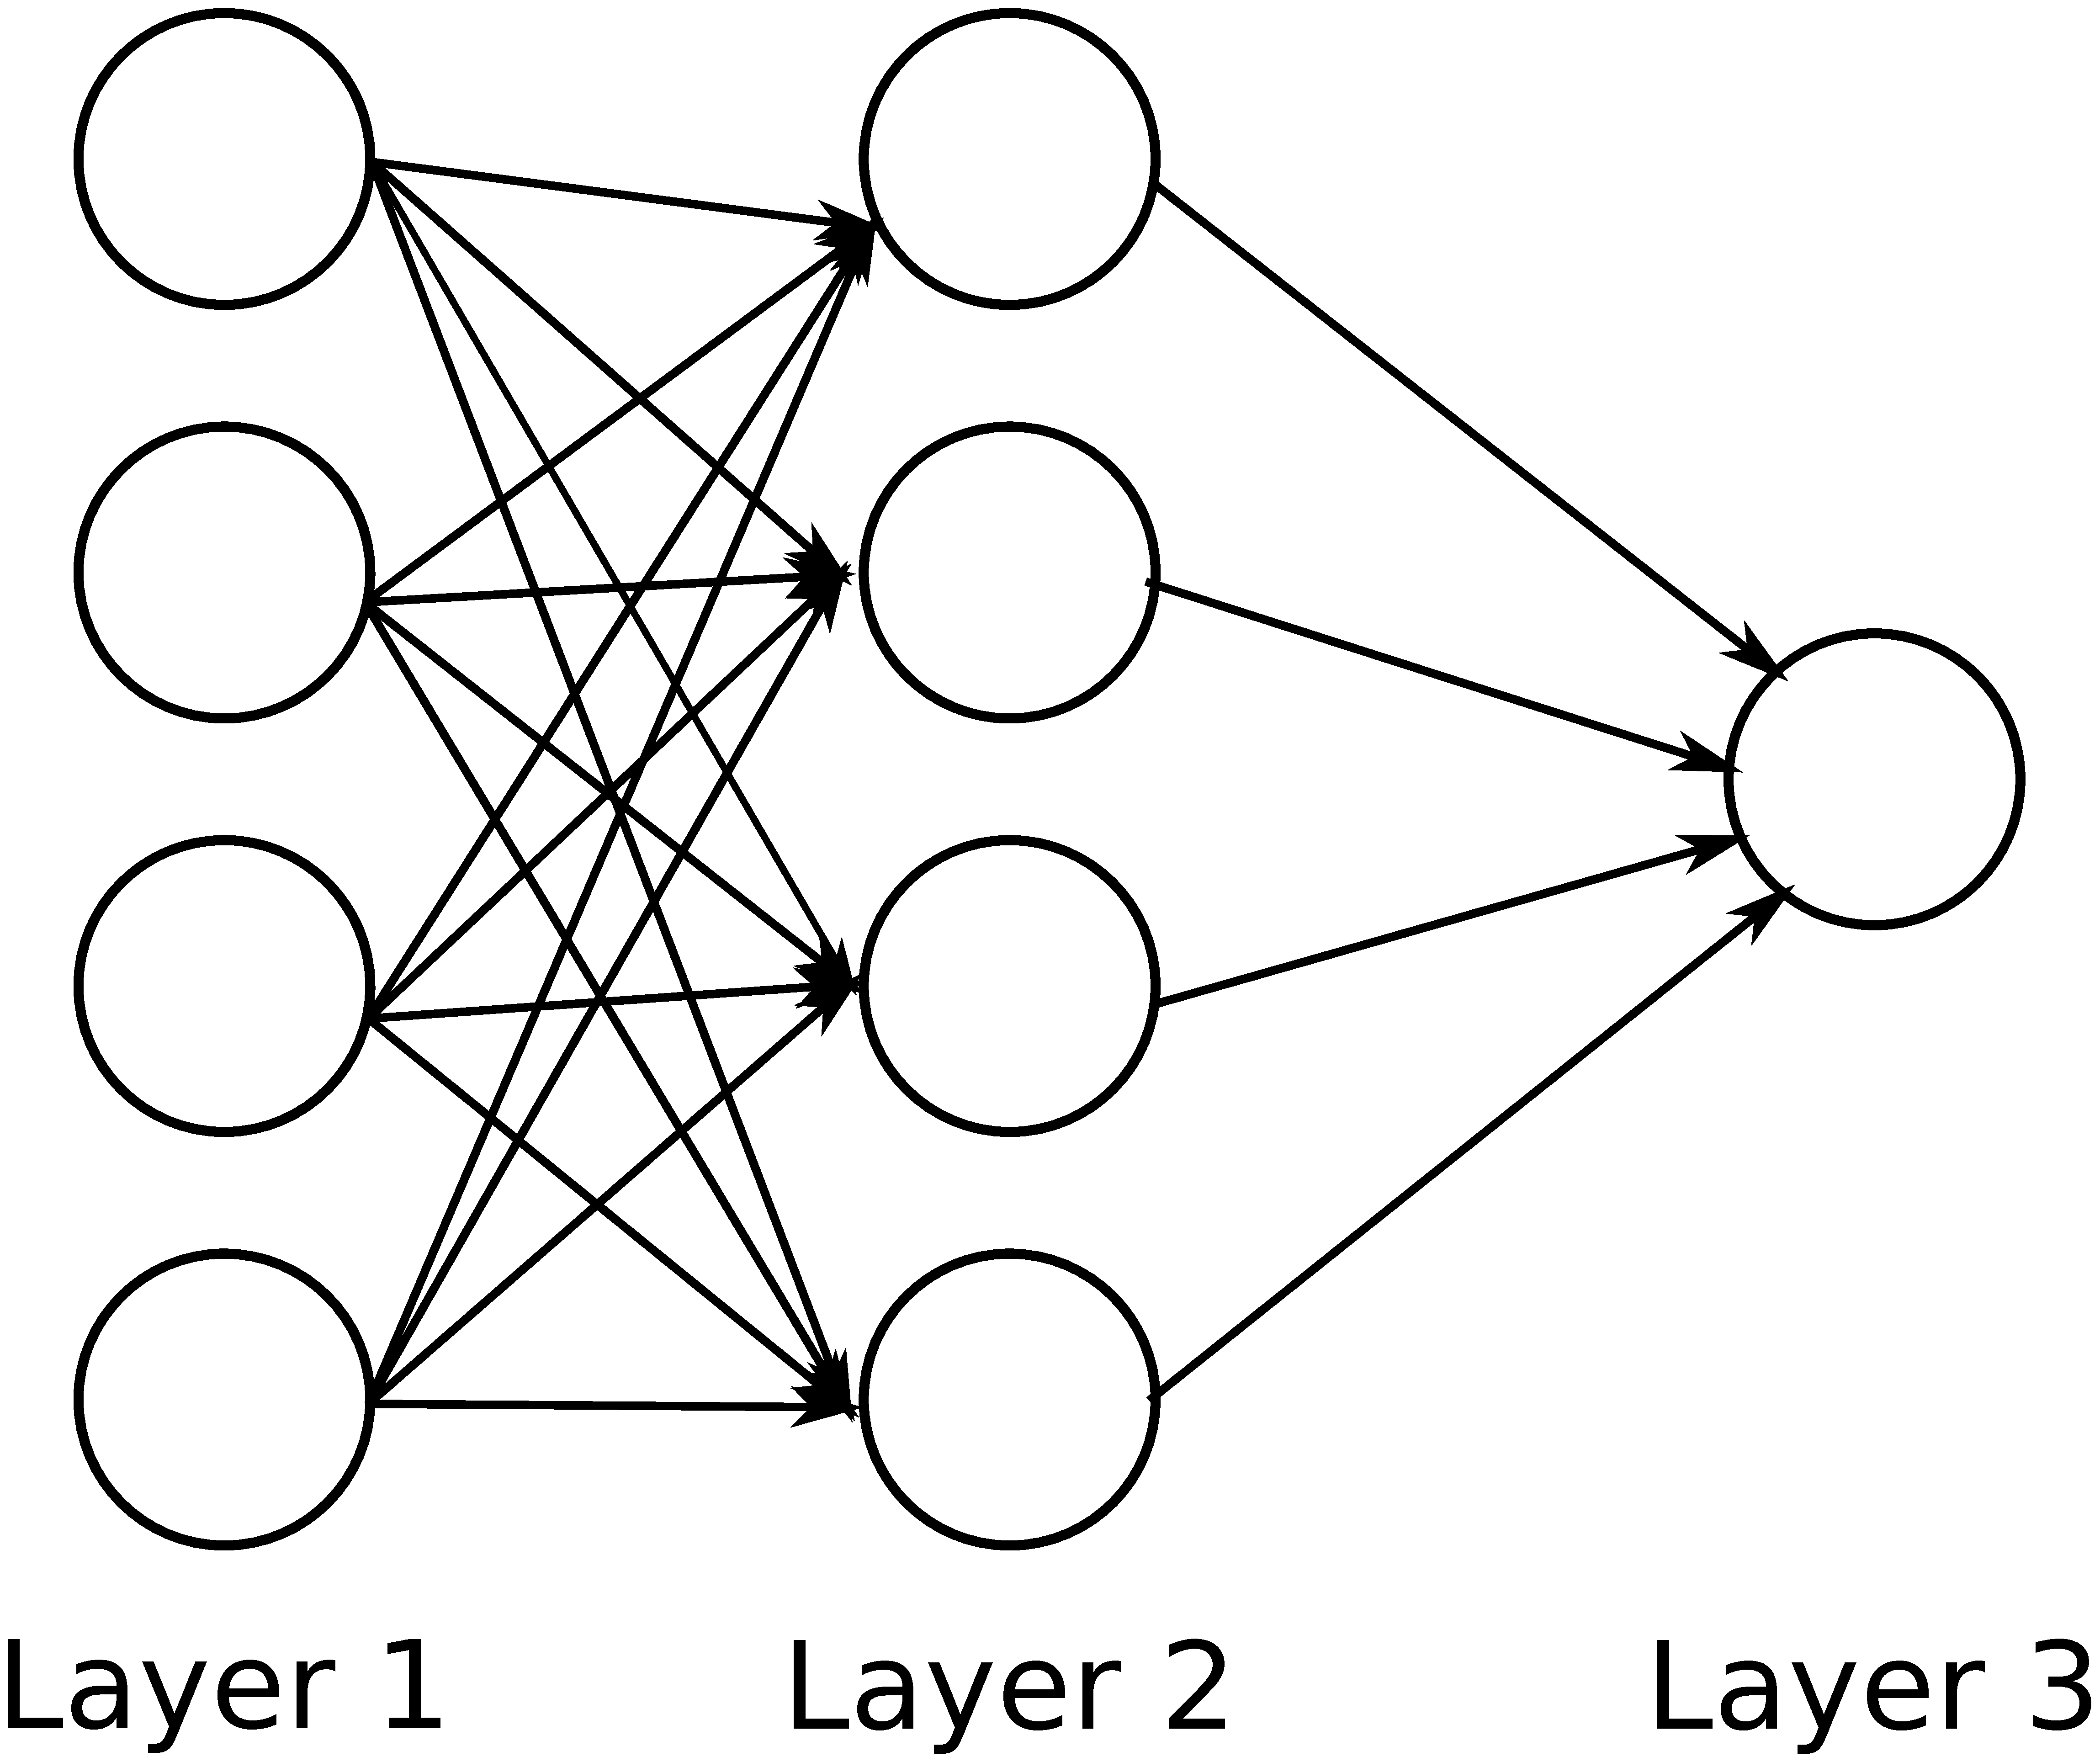
\includegraphics[scale=0.05]{network.eps}
        \label{fig:my_label}
    \end{figure}
    \vspace{0.3cm}
    \begin{center}
     $z_j^L = \omega_{jk}^L a_k^{L-1} + b_k$\\
        $a_j^L = \sigma ( z_j^L )$
    \end{center}
    \end{column}
\end{columns}
\end{frame}

\begin{frame}{Neural Networks}
\begin{figure}
    \centering
    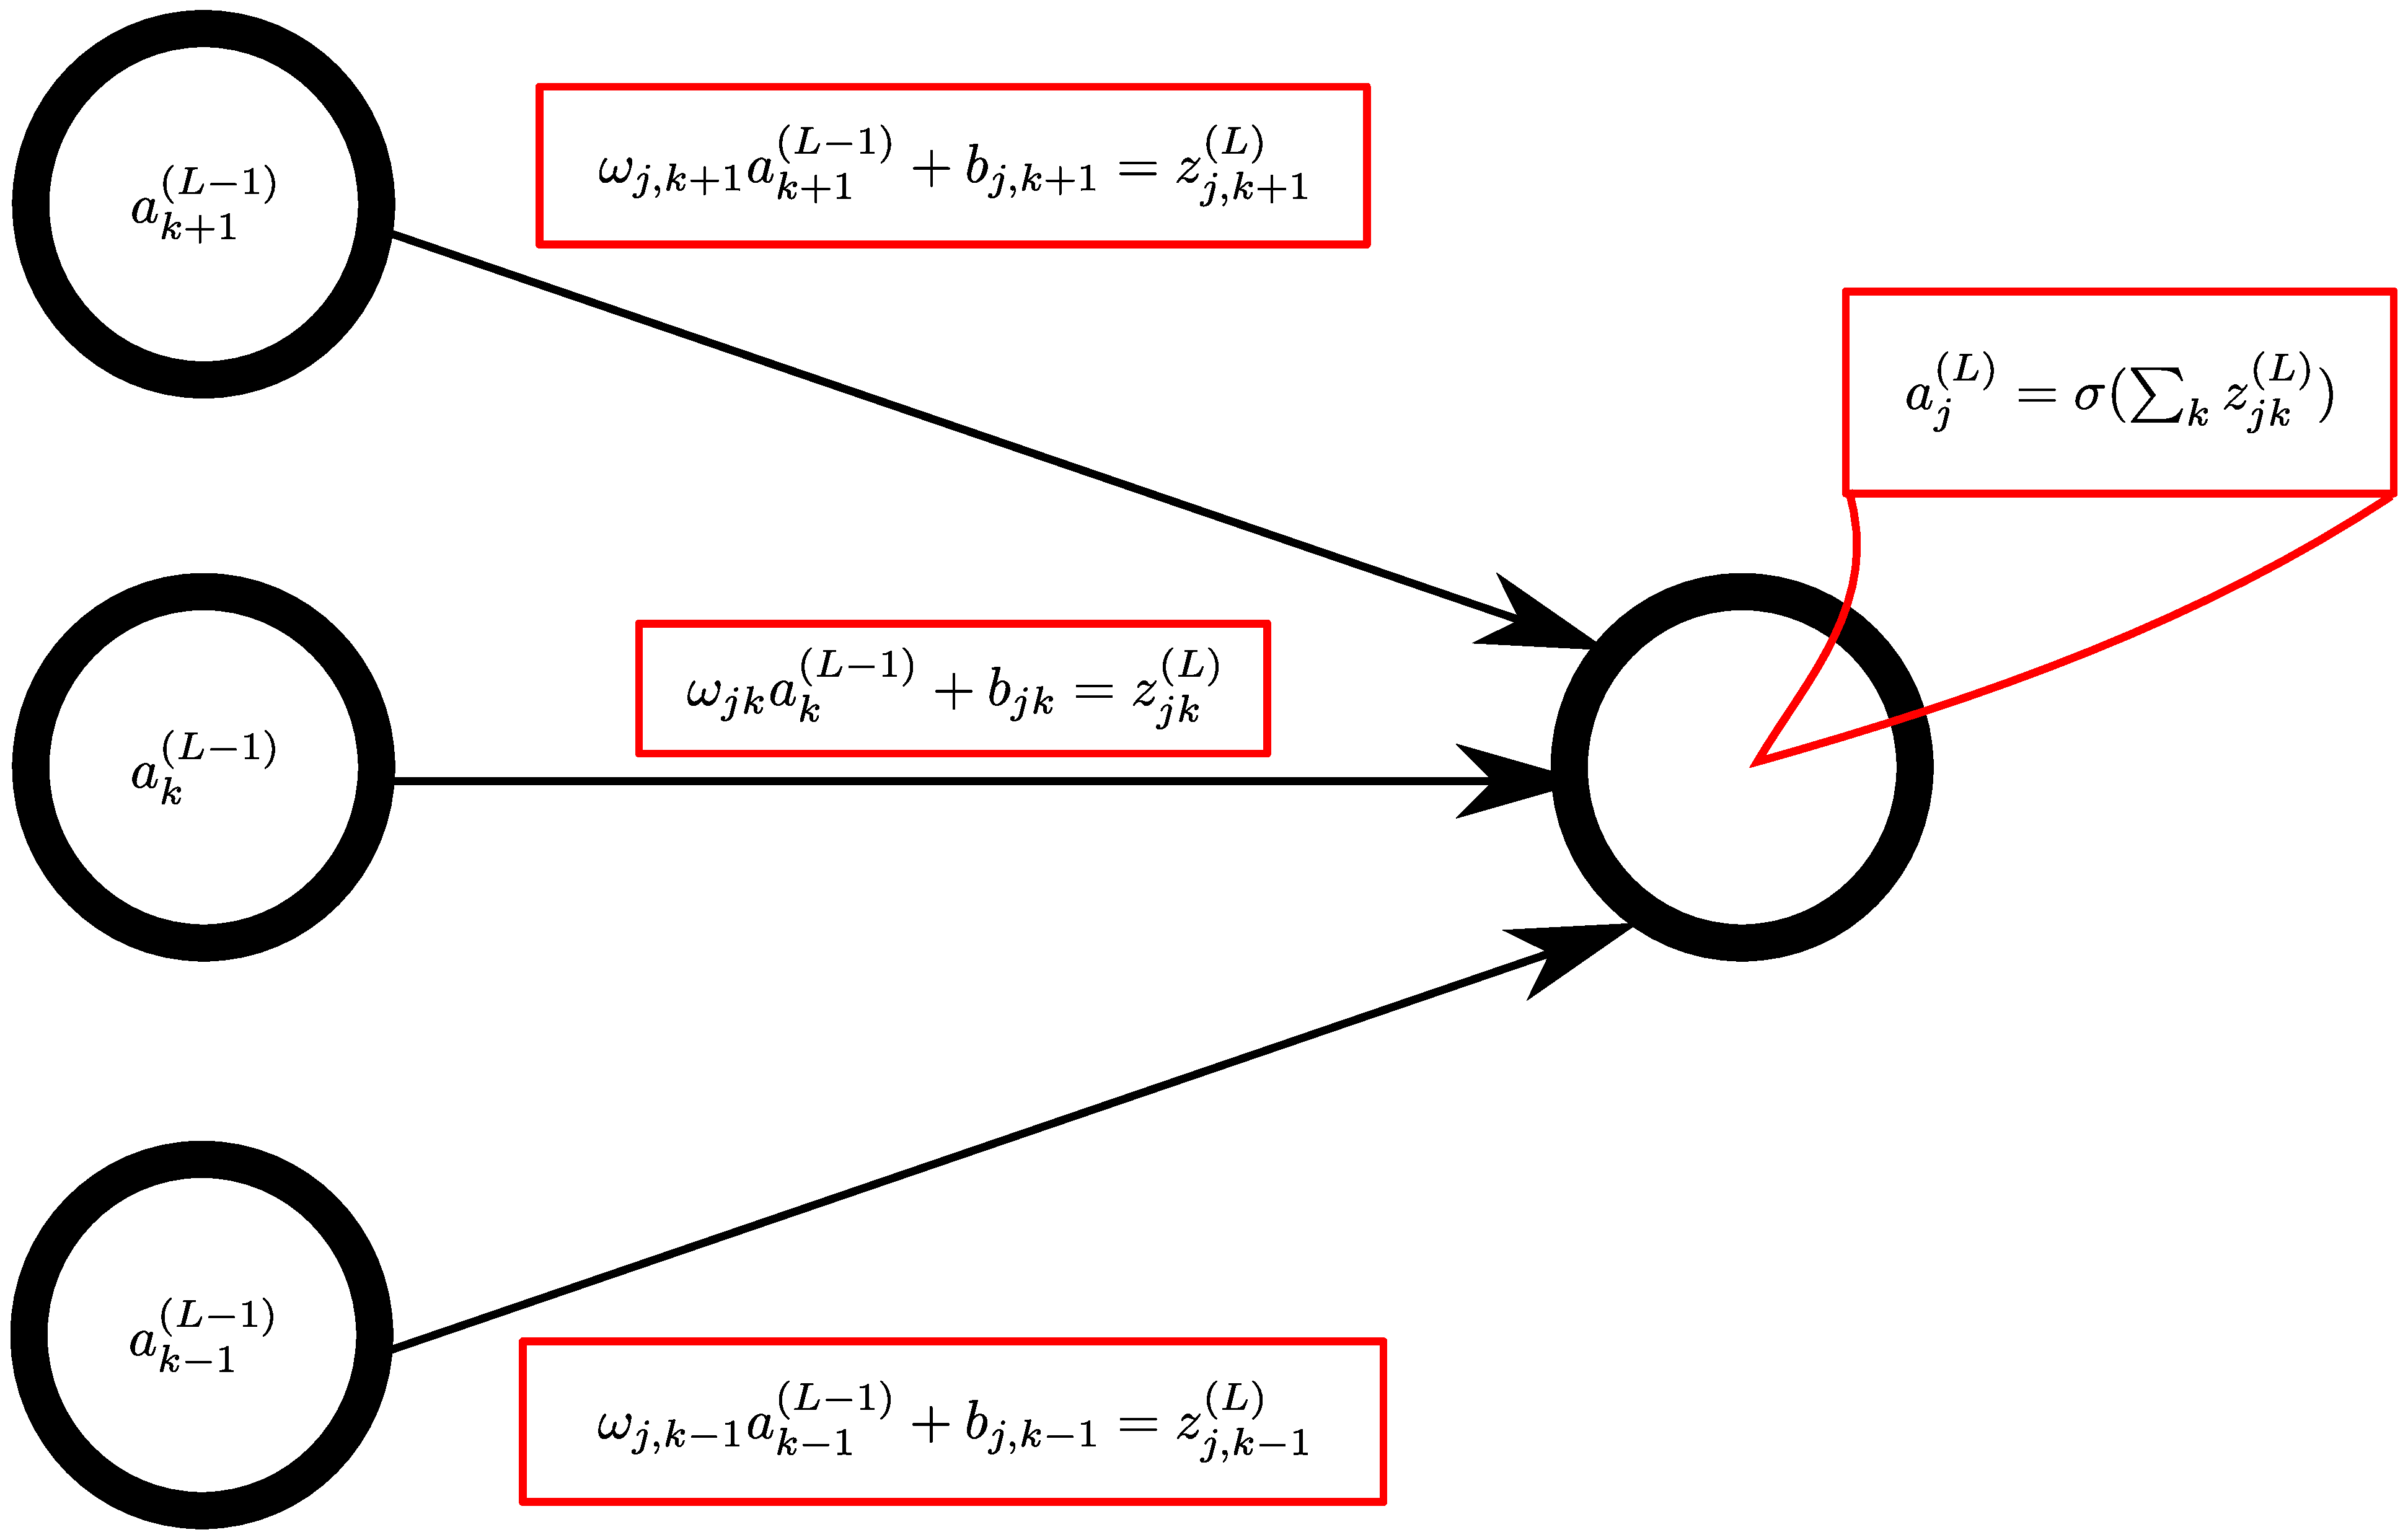
\includegraphics[scale=0.15]{nodes_nomenclature.eps}
    \caption{Forward Propagation in a neural network}
    \label{fig:my_label}
\end{figure}
\end{frame}

\begin{frame}{Choosing the next step}
    \begin{itemize}
        \item In supervised learning truth tagged training data allows to calculate a cost function to estimate a model's quality. For example crossentropy:
        \begin{align}
            C = -(y \log p + (1 - y) \log (1 - p) )
            \label{eq:binary_crossentropy}
        \end{align}
        \item Backpropagation estimates the parameters' impact on the cost function using the partial derivatives
        \begin{align*}
            \frac{\partial C}{\partial a_k^{L-1}} = \sum_{j=1}^N \frac{\partial z_j^L}{\partial a_k^{L-1}} \frac{\partial a_j^L}{\partial z_j^L}\frac{\partial C}{\partial a_j^L}
        \end{align*}
        \item Each parameter is then updated accoring to its impact on the cost function
    \end{itemize}
\end{frame}


\begin{frame}{Adversarial Neural Networks}
    \begin{itemize}
        \item Originally introduced as Generative adversarial neural networks to overcome weaknesses of generative networks \cite{2014arXiv1406.2661G}
        \item Adds a second network controlling the dependency on features with large systematic uncertainties. 
        \item The adversarial structure of the networks creates a minimax game
        \item Combined loss function
    \end{itemize}
\end{frame}

\begin{frame}{Optimisers}
\begin{itemize}
    \item Gradient Descent: Update parameters in the opposite direction of the error gradient
    \item Stochastic Gradient Descent: Gradient Descent but for each training example separately
    \item Adaptive Moment Estimation, Adam: adaptive learning rate based on exponentially decaying mean of past gradients and past square gradients.
    \item Others
    \item https://towardsdatascience.com/types-of-optimization-algorithms-used-in-neural-networks-and-ways-to-optimize-gradient-95ae5d39529f
\end{itemize}
    
\end{frame}



\begin{frame}{Learning rate, momentum, decay}
\begin{itemize}
    \item Learning rate: Step-length in gradient direction
    \begin{align}
    \theta^{\prime} = \theta - lr \cdot g
    \end{align}
    \item Momentum: create an adaptive and weight dependent learning rate
    \begin{align}
    \nu^{\prime} = \alpha \nu - \epsilon \frac{1}{m} \nabla_{\theta} \sum_j L(f(\hat{y}^j; \theta), y^j)\\
    \theta^{\prime} = \theta + \nu
    \end{align}
    \item Decay: Decrease the learning rate over the course of the training
    \begin{align}
    \epsilon^{\prime} = \frac{\epsilon}{1 + \phi t}
    \end{align}
\end{itemize}
\end{frame}


\begin{frame}{Dropout}
\begin{figure}
    \centering
    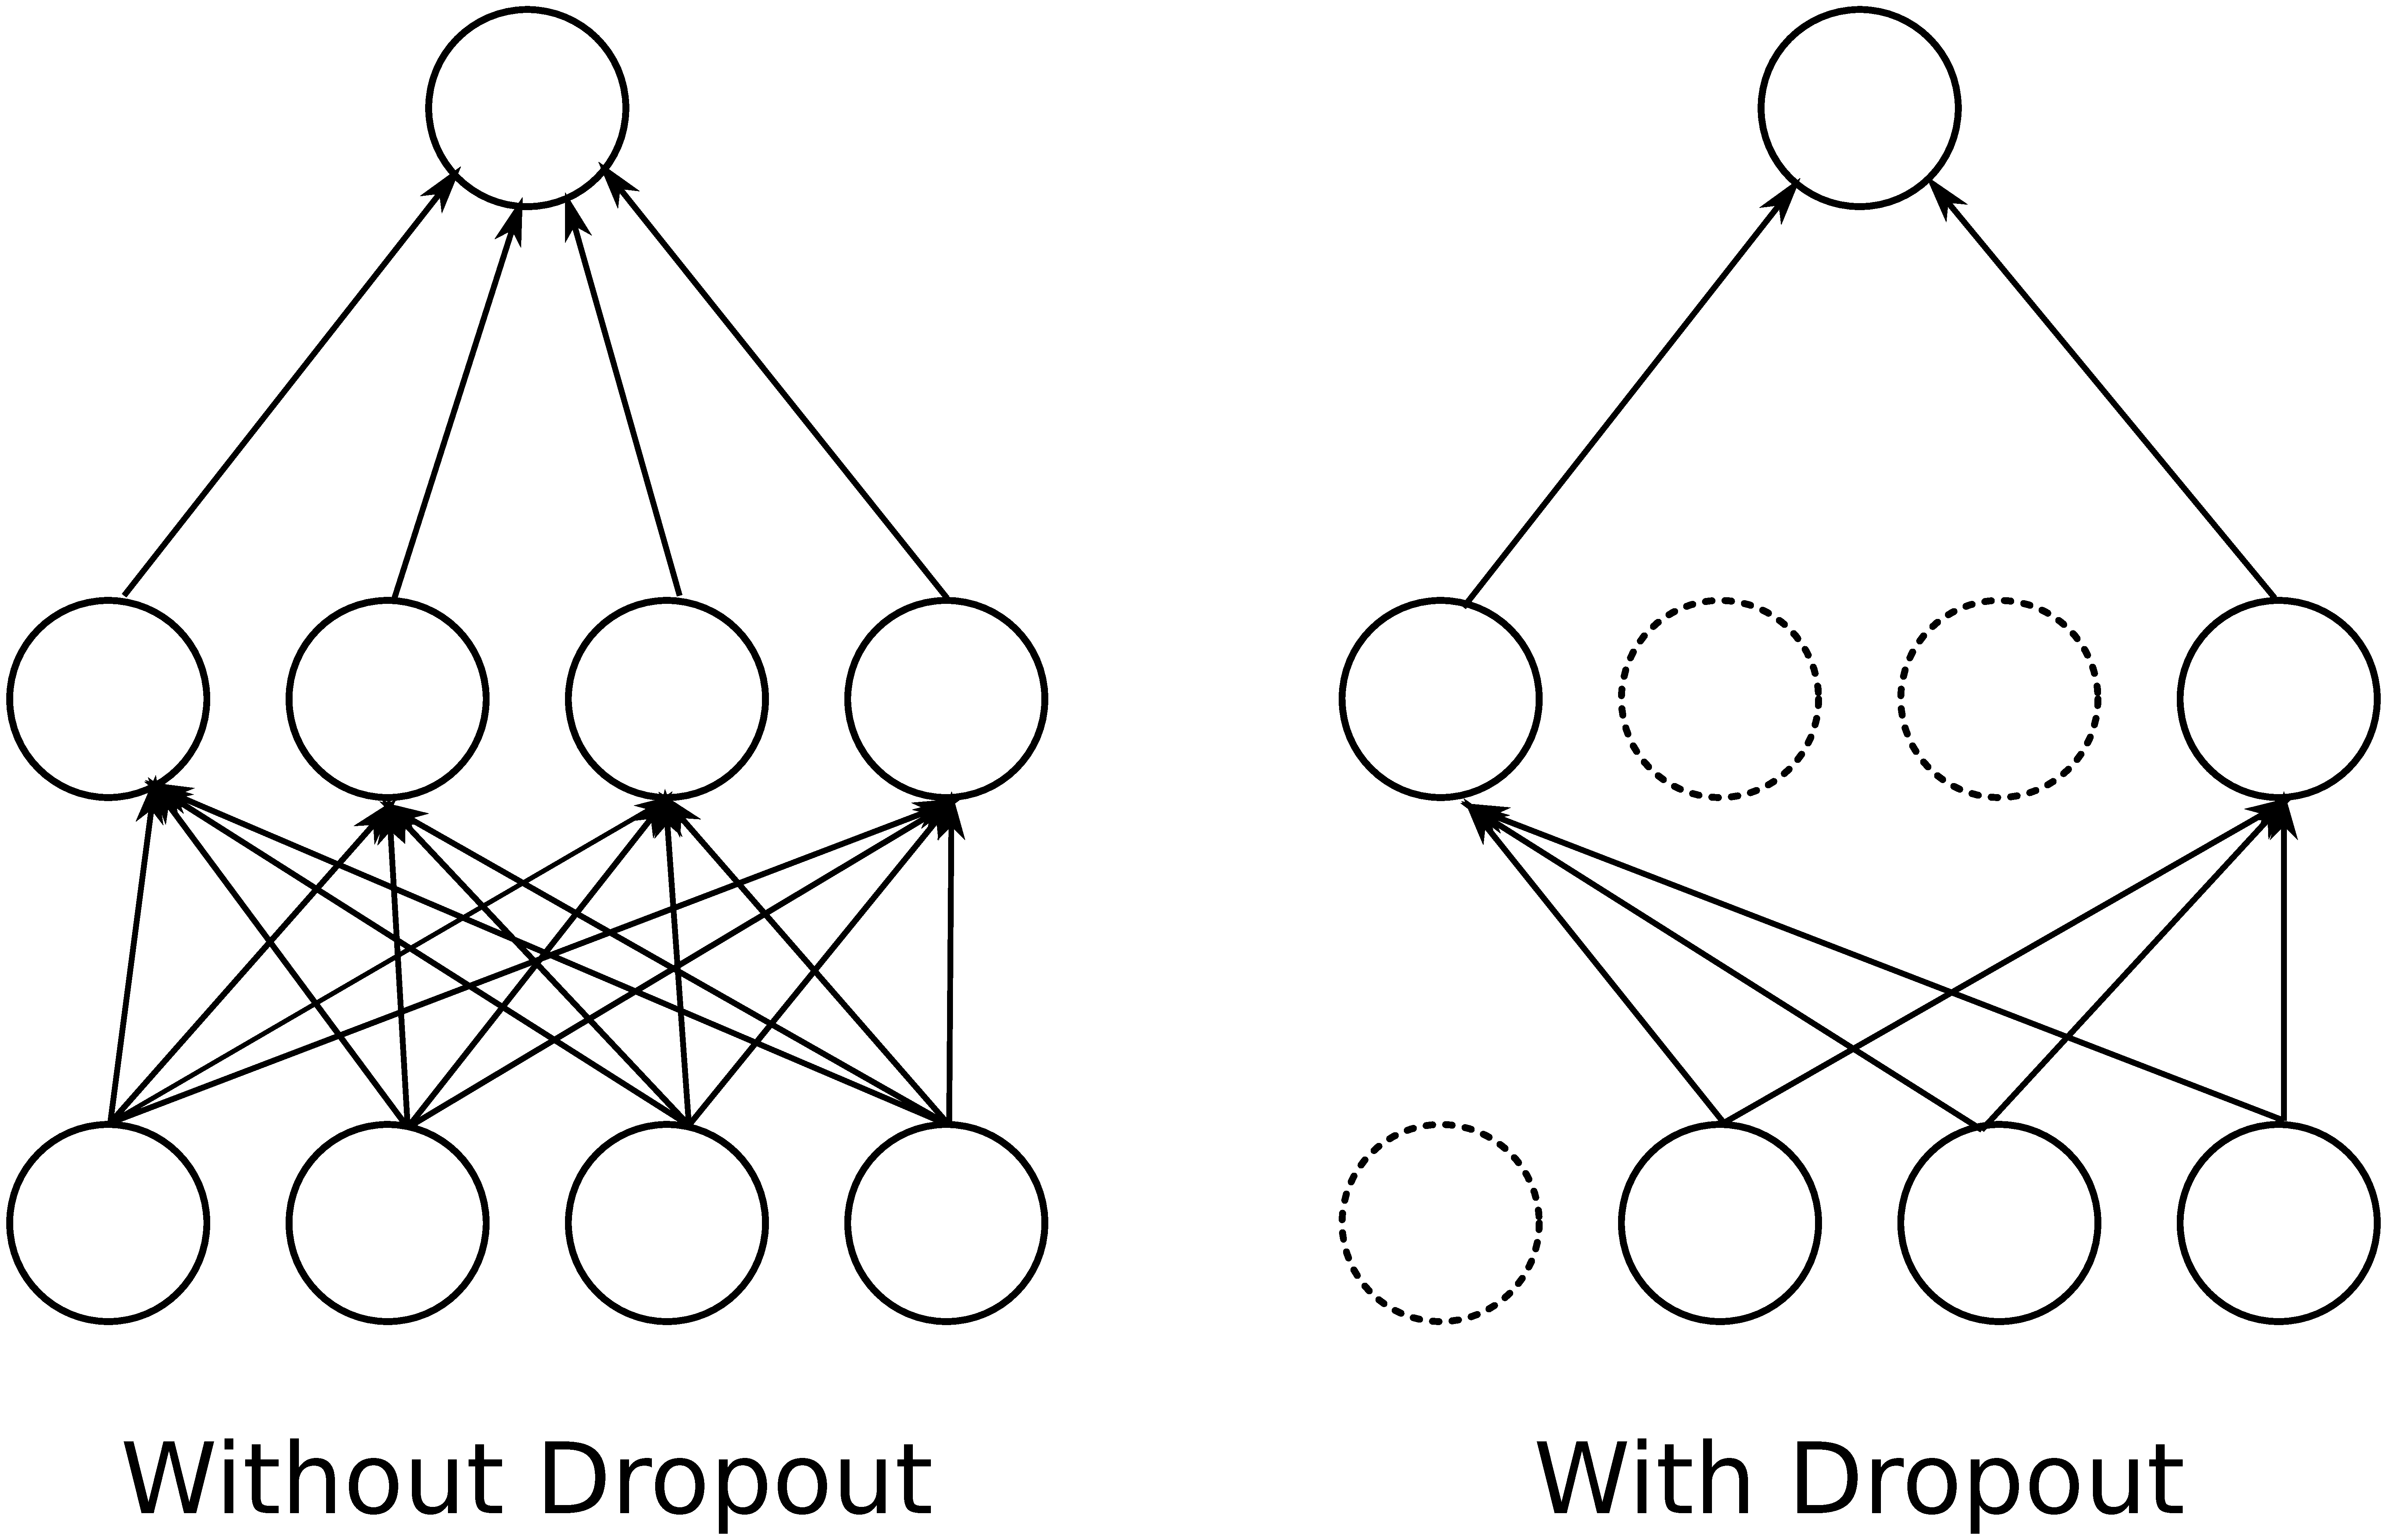
\includegraphics[scale=0.07]{dropout.eps}
    \caption{Caption}
    \label{fig:my_label}
\end{figure}
\end{frame}

\begin{frame}{Technical details}
    \begin{itemize}
        \item The neural networks were built using Keras \cite{chollet2015keras} with tensorflow \cite{tensorflow2015-whitepaper} as backend
    \end{itemize}
\end{frame}

\begin{frame}{Variables}
Inhalt...
\end{frame}